
\subsection{link-analysis}

\begin{figure}[h!]
    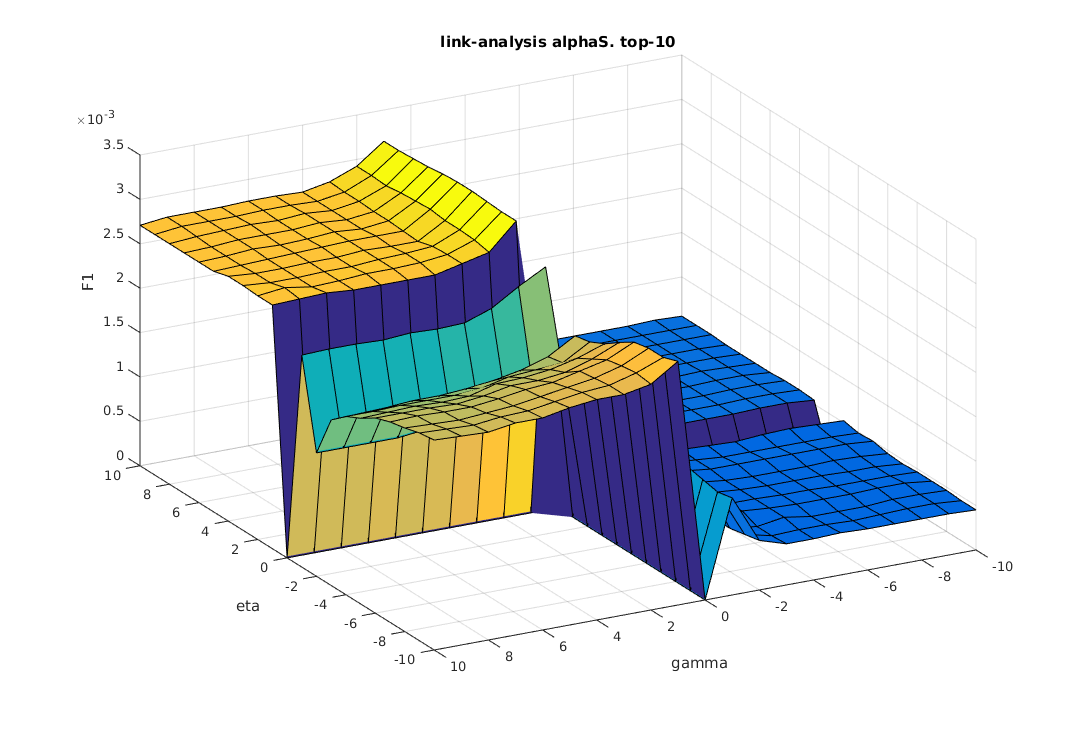
\includegraphics[width=\textwidth]{fig/link_eta_gamma/alphaS_link_eta.png}
    \caption{\textit{alphaS}}
\end{figure}

\begin{figure}[h!]
\centering
\begin{minipage}{.5\textwidth}
    \centering
    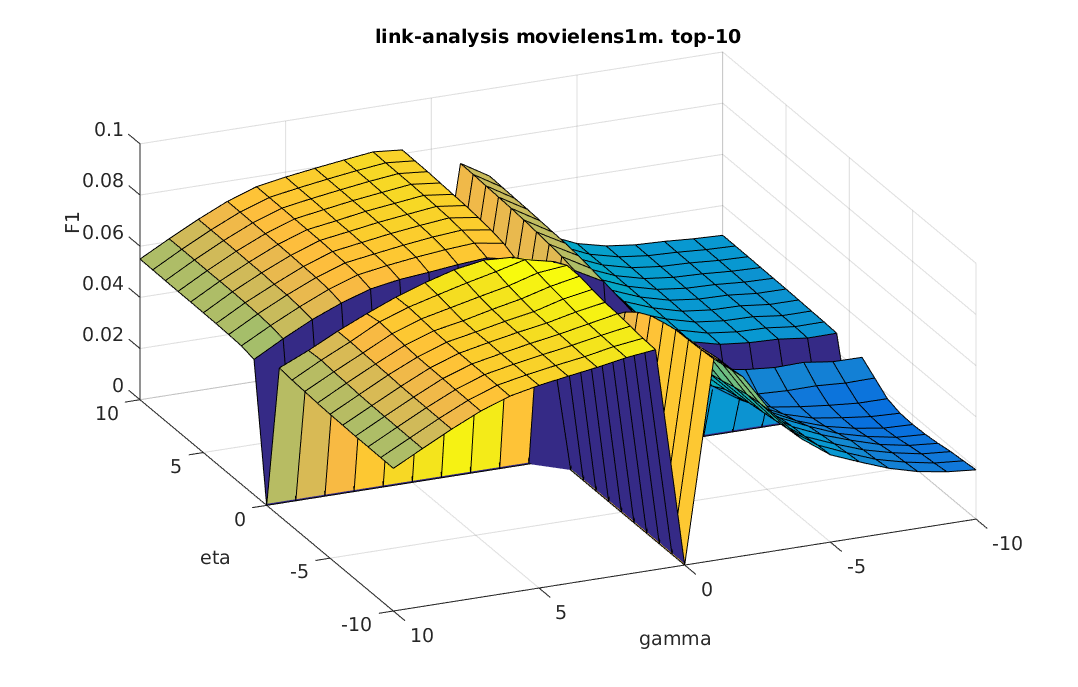
\includegraphics[width=\linewidth]{fig/link_eta_gamma/movielens_link_eta.png}
    \captionof{figure}{\textit{movielens1m}}
\end{minipage}%
\begin{minipage}{.5\textwidth}
    \centering
    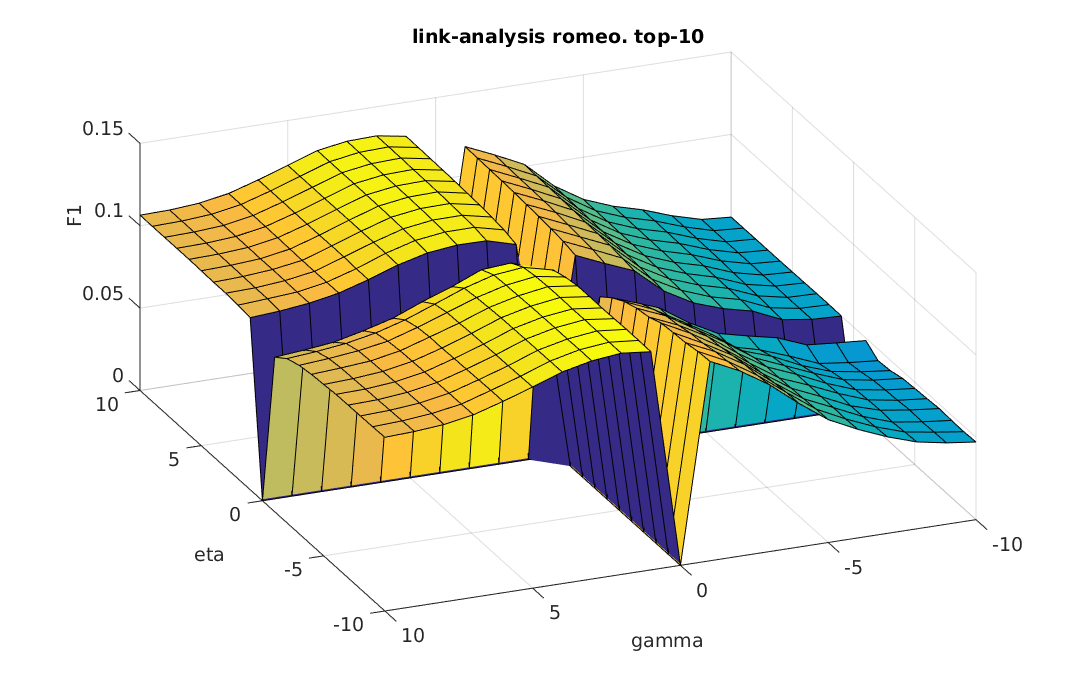
\includegraphics[width=\linewidth]{fig/link_eta_gamma/romeo_link_eta.png}
    \captionof{figure}{\textit{romeo}}
\end{minipage}
\end{figure}

\FloatBarrier

\begin{figure}[h!]
    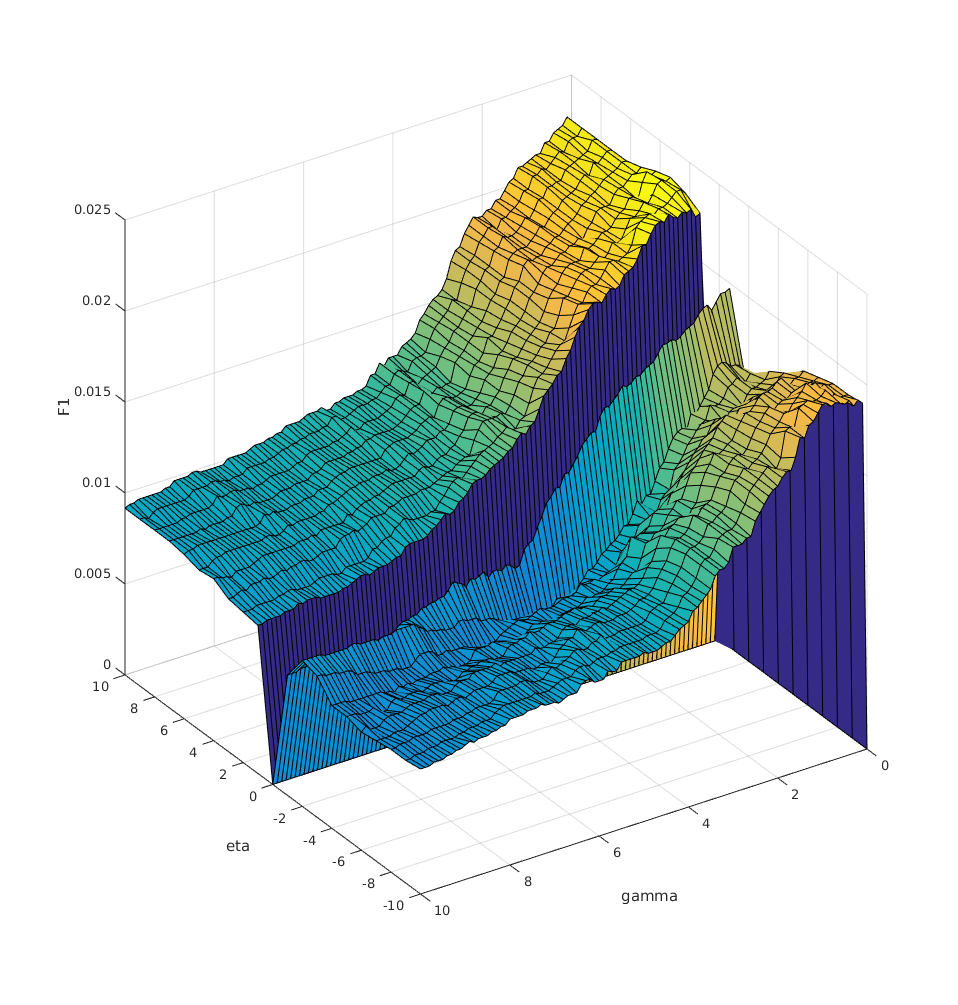
\includegraphics[width=\textwidth]{fig/link_eta_gamma/eswc2015books.png}
    \caption{\textit{eswc2015books}}
\end{figure}

\FloatBarrier

A closer look at \textit{eswc2015books} reveal that the function space isn't as smooth as it might have seemed in the previous plots, several local optima can be seen. The function space if viewed with a lower level of detail is still fairly smooth and convex, with the exception of $eta = 0$.

\newpage

Then some comments of eta... Some have eta > 0 as their biggest value, and some have eta < 0.

\FloatBarrier

\begin{figure}[h!]
\centering
\begin{minipage}{.5\textwidth}
    \centering
    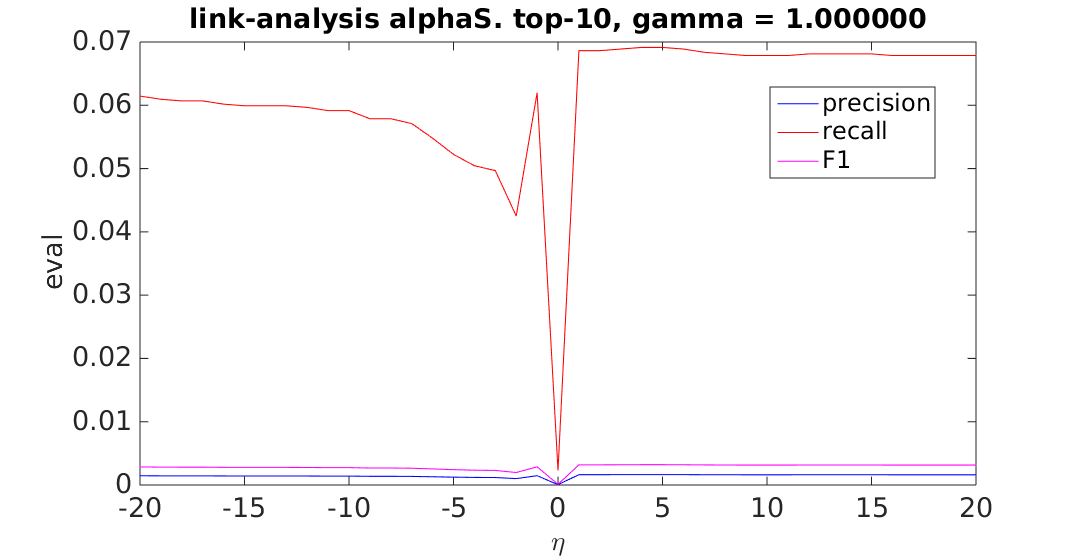
\includegraphics[width=\linewidth]{fig/link_eta/alphaS_link_eta.png}
    \captionof{figure}{\textit{alphaS}}
\end{minipage}%
\begin{minipage}{.5\textwidth}
    \centering
    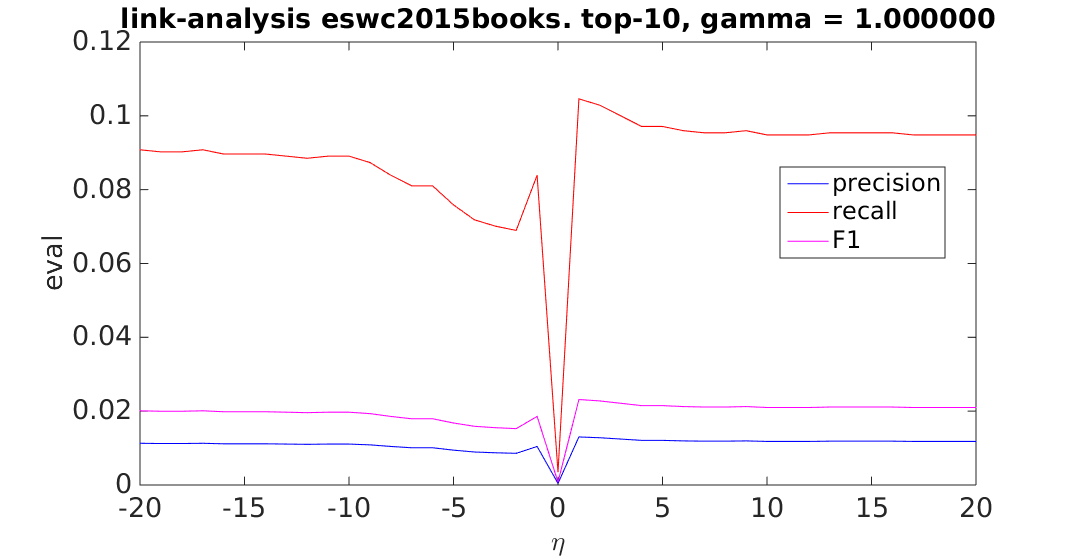
\includegraphics[width=\linewidth]{fig/link_eta/eswc2015books_link_eta.png}
    \captionof{figure}{\textit{eswc2015books}}
\end{minipage}
\end{figure}

\begin{figure}[h!]
\centering
\begin{minipage}{.5\textwidth}
    \centering
    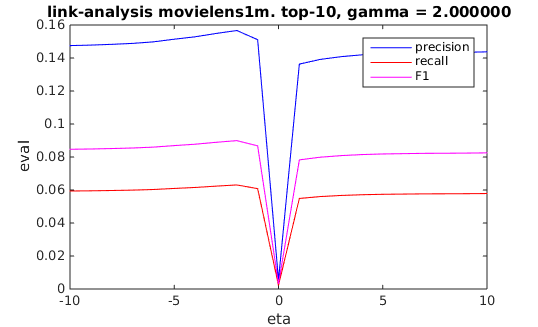
\includegraphics[width=\linewidth]{fig/link_eta/movielens_link_eta.png}
    \captionof{figure}{\textit{movielens1m}}
\end{minipage}%
\begin{minipage}{.5\textwidth}
    \centering
    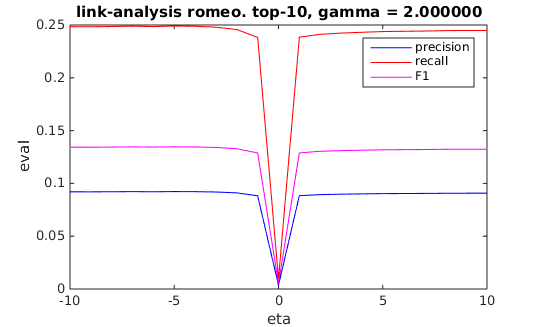
\includegraphics[width=\linewidth]{fig/link_eta/romeo_link_eta.png}
    \captionof{figure}{\textit{romeo}}
\end{minipage}
\end{figure}

\FloatBarrier

\newpage

And some comments of gamma... This seems to be the important parameter which varies the most!

\FloatBarrier

\begin{figure}[h!]
\centering
\begin{minipage}{.5\textwidth}
    \centering
    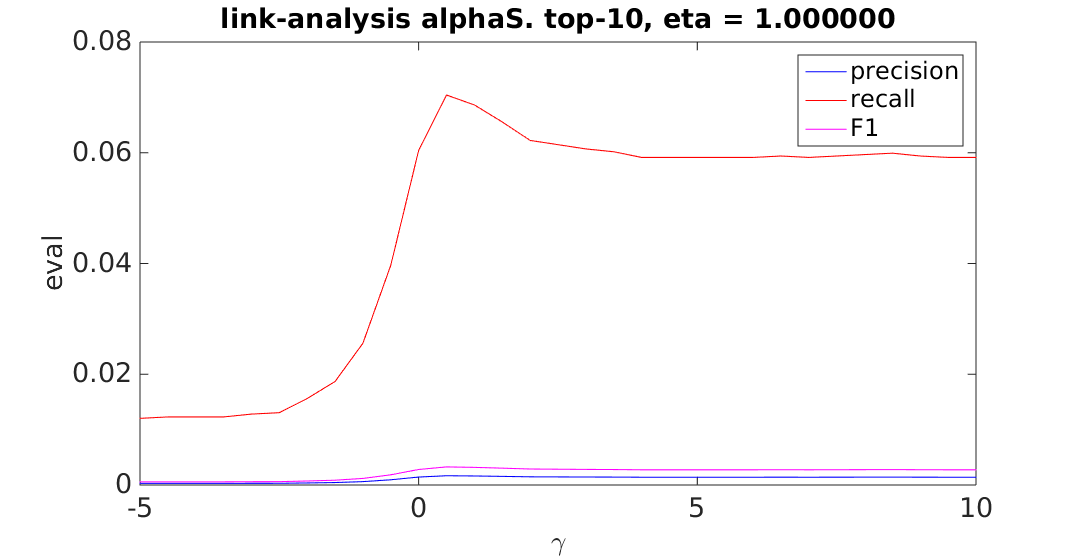
\includegraphics[width=\linewidth]{fig/link_gamma/alphaS_link_gamma.png}
    \captionof{figure}{\textit{alphaS}}
\end{minipage}%
\begin{minipage}{.5\textwidth}
    \centering
    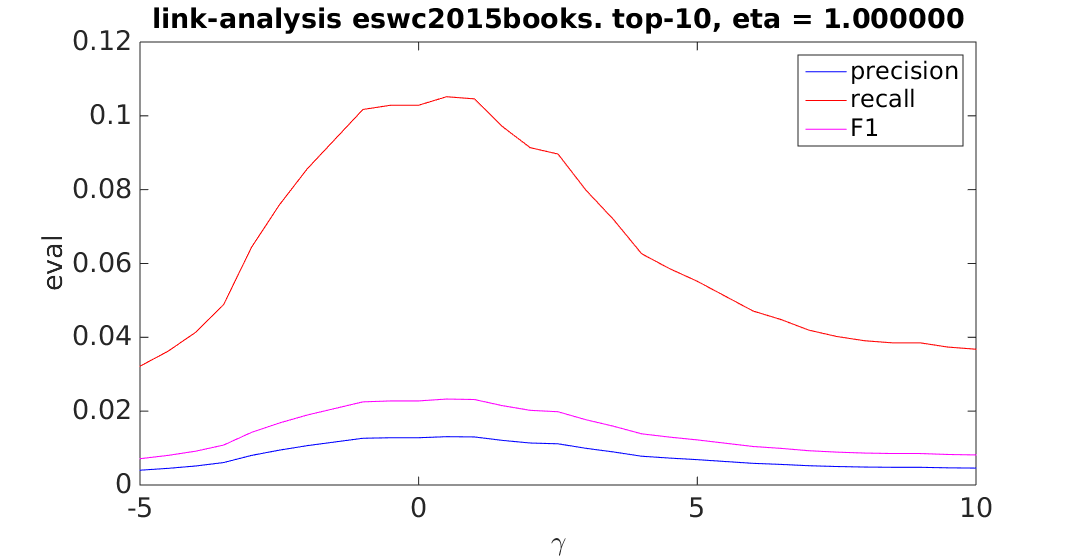
\includegraphics[width=\linewidth]{fig/link_gamma/eswc2015books_link_gamma.png}
    \captionof{figure}{\textit{eswc2015books}}
\end{minipage}
\end{figure}

\begin{figure}[h!]
\centering
\begin{minipage}{.5\textwidth}
    \centering
    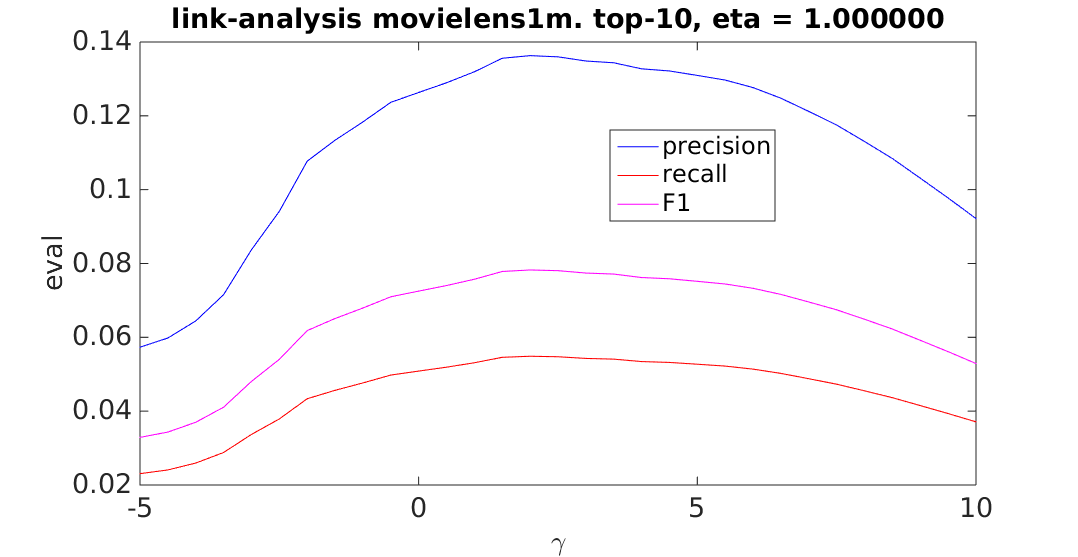
\includegraphics[width=\linewidth]{fig/link_gamma/movielens_link_gamma.png}
    \captionof{figure}{\textit{movielens1m}}
\end{minipage}%
\begin{minipage}{.5\textwidth}
    \centering
    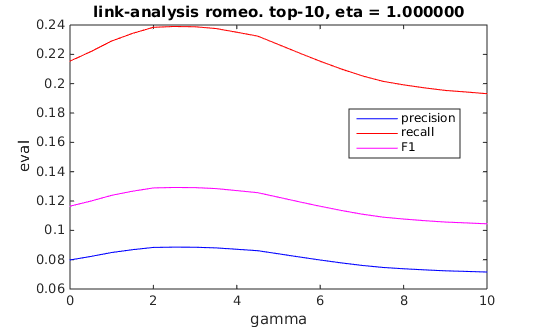
\includegraphics[width=\linewidth]{fig/link_gamma/romeo_link_gamma.png}
    \captionof{figure}{\textit{romeo}}
\end{minipage}
\end{figure}

\FloatBarrier
